\begin{frame}
\frametitle{Brisbane}
\begin{center}
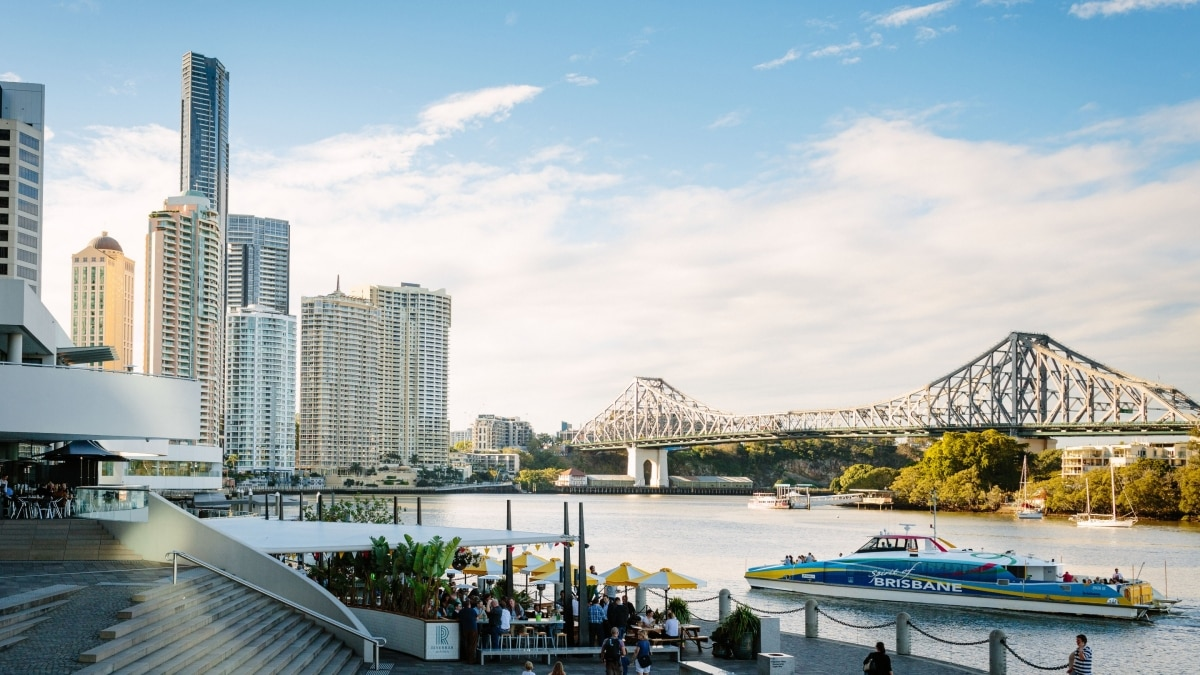
\includegraphics[width=0.9\textwidth]{image/brisbane.jpg}
\end{center}
\end{frame}

\begin{frame}
\frametitle{Queensland}
\begin{center}

\includegraphics[width=0.9\textwidth]{image/queensland.jpg}
\end{center}
\end{frame}

\begin{frame}
\frametitle{Brisbane east coast}
\begin{center}
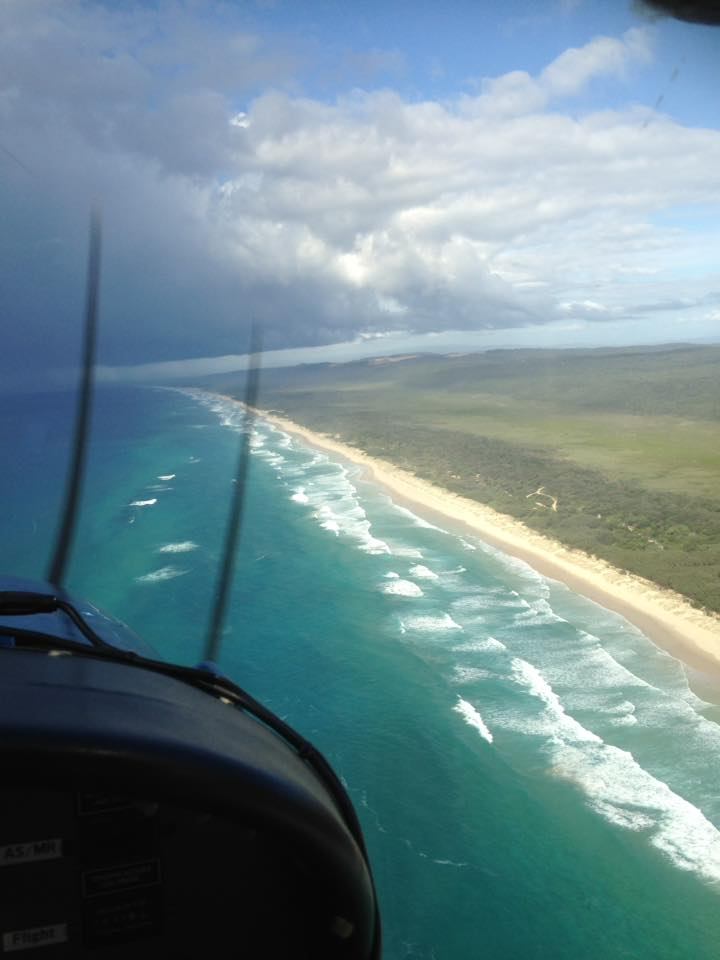
\includegraphics[width=0.5\textwidth]{image/20180420-vh-afr_00.jpg}
\end{center}
\end{frame}

\begin{frame}
\frametitle{QFPL}
\begin{center}
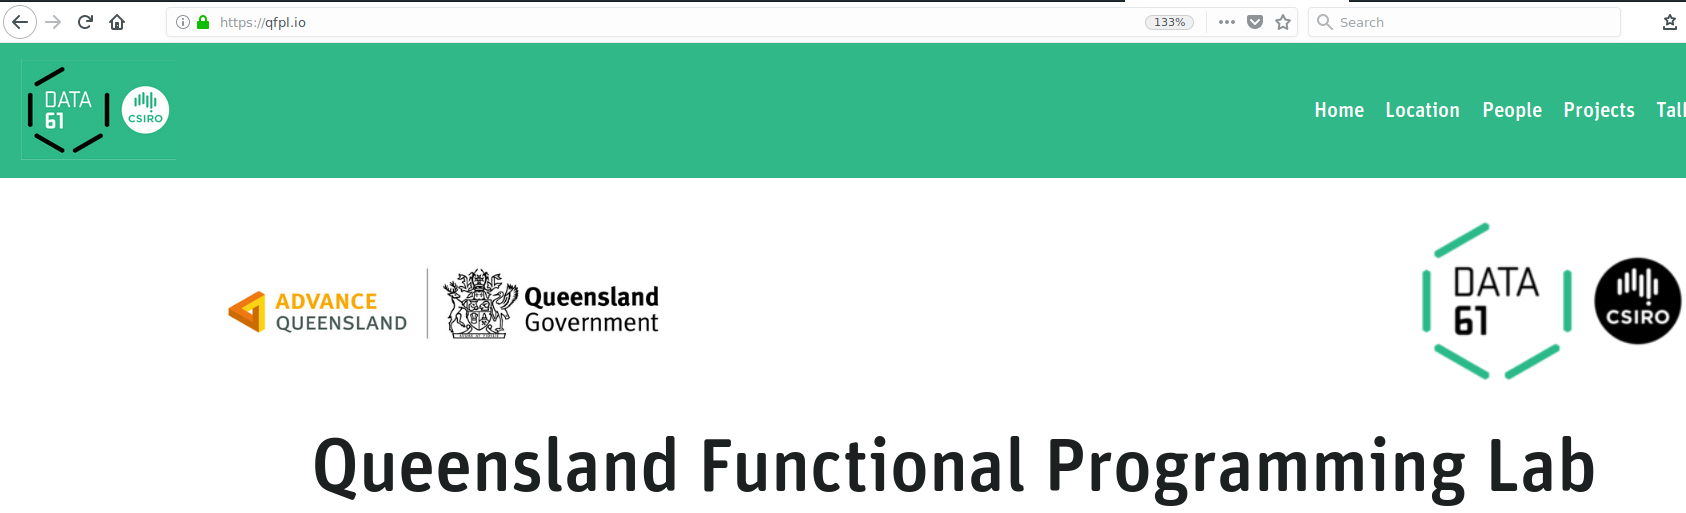
\includegraphics[width=0.9\textwidth]{image/qfpl_io.png}
\end{center}
\end{frame}

\begin{frame}
\frametitle{Intro}
\begin{block}{Explain List Folds to Yourself, April 2013}
In April 2013, BFPG had a chat about list folds
\includegraphics[height=0.5\textheight]{image/list-folds-2013.png}
\end{block}
\end{frame}

\begin{frame}
\frametitle{Introduction}
\begin{block}{Today}
\begin{itemize}
\item<1-> we are doing a similar thing, with differences
\item<2-> aiming to beginners, who have only had cursory experiences with lists
\item<3-> being very explicit about the utility of the developed intuition, and developing it further
\end{itemize}
\end{block}
\end{frame}
